\documentclass[aspectratio=169]{beamer}

% Theme and colors
\usetheme{Madrid}
\usecolortheme{whale}
\setbeamertemplate{navigation symbols}{}
\setbeamertemplate{footline}[frame number]

% Packages
\usepackage[utf8]{inputenc}
\usepackage[T1]{fontenc}
\usepackage{graphicx}
\usepackage{booktabs}
\usepackage{tikz}
\usepackage{hyperref}

% Custom colors
\definecolor{fakered}{RGB}{255, 107, 107}
\definecolor{realgreen}{RGB}{81, 207, 102}
\definecolor{primaryblue}{RGB}{102, 126, 234}

% Title information
\title[Fake News Classifier]{Fake News Classification System}
\subtitle{NLP-based Classification using Deep Learning}
\author{Fake News Classifier Project}
\date{December 2025}
\institute{Machine Learning \& NLP}

\begin{document}

% ============================================================================
% SLIDE 1: Title
% ============================================================================
\begin{frame}
    \titlepage
\end{frame}

% ============================================================================
% SLIDE 2: Project Overview
% ============================================================================
\begin{frame}{Project Overview}
    \begin{columns}
        \begin{column}{0.5\textwidth}
            \textbf{Goal:}
            \begin{itemize}
                \item Automated fake news detection
                \item Multiple model comparison
                \item Production-ready web interface
            \end{itemize}
            
            \vspace{0.5cm}
            \textbf{Target Audience:}
            \begin{itemize}
                \item Journalists \& Fact-checkers
                \item Content Moderators
                \item Researchers
            \end{itemize}
        \end{column}
        \begin{column}{0.5\textwidth}
            \textbf{Technology Stack:}
            \begin{itemize}
                \item \textbf{Backend:} FastAPI (Python)
                \item \textbf{Frontend:} HTML5/CSS3/JS
                \item \textbf{ML:} PyTorch
                \item \textbf{Models:} LSTM, CNN, BERT, DistilBERT
                \item \textbf{Deploy:} Railway + GitHub Pages
            \end{itemize}
        \end{column}
    \end{columns}
\end{frame}

% ============================================================================
% SLIDE 3: Datasets
% ============================================================================
\begin{frame}{Datasets}
    \begin{columns}
        \begin{column}{0.5\textwidth}
            \textbf{ISOT/Kaggle Dataset}
            \begin{itemize}
                \item 44,898 articles total
                \item Fake: 23,481 (52.3\%)
                \item Real: 21,417 (47.7\%)
                \item Avg length: $\sim$2,400 chars
            \end{itemize}
        \end{column}
        \begin{column}{0.5\textwidth}
            \textbf{LIAR Dataset}
            \begin{itemize}
                \item 12,791 political statements
                \item 6-level $\rightarrow$ binary labels
                \item Rich metadata (speaker, party)
                \item Avg length: $\sim$107 chars
            \end{itemize}
        \end{column}
    \end{columns}
    
    \vspace{0.5cm}
    \centering
    \textbf{Data Split:} Train 64\% | Validation 16\% | Test 20\%
    
    \vspace{0.3cm}
    \small{Stratified split to preserve class balance}
\end{frame}

% ============================================================================
% SLIDE 4: Model Architectures
% ============================================================================
\begin{frame}{Model Architectures}
    \begin{columns}
        \begin{column}{0.5\textwidth}
            \textbf{Baseline Models:}
            
            \vspace{0.3cm}
            \underline{CNN-Text}
            \begin{itemize}
                \item GloVe 100d embeddings
                \item 1D Conv filters [3,4,5]
                \item Global Max Pooling
                \item $\sim$1-2M parameters
            \end{itemize}
            
            \vspace{0.3cm}
            \underline{Bidirectional LSTM}
            \begin{itemize}
                \item GloVe 100d embeddings
                \item Hidden dim: 128
                \item Dropout: 0.3
                \item $\sim$500K-1M parameters
            \end{itemize}
        \end{column}
        \begin{column}{0.5\textwidth}
            \textbf{Transformer Models:}
            
            \vspace{0.3cm}
            \underline{BERT-base-uncased}
            \begin{itemize}
                \item 12 transformer layers
                \item Fine-tuned for classification
                \item High accuracy
            \end{itemize}
            
            \vspace{0.3cm}
            \underline{DistilBERT}
            \begin{itemize}
                \item 6 transformer layers
                \item 40\% smaller than BERT
                \item Similar accuracy, faster
            \end{itemize}
        \end{column}
    \end{columns}
\end{frame}

% ============================================================================
% SLIDE 5: Training Configuration
% ============================================================================
\begin{frame}{Training Configuration}
    \begin{columns}
        \begin{column}{0.5\textwidth}
            \textbf{Hyperparameters:}
            \begin{itemize}
                \item Batch size: 16
                \item Learning rate: 2e-5
                \item Max epochs: 10
                \item Early stopping: patience=3
                \item Gradient clipping: 1.0
            \end{itemize}
            
            \vspace{0.3cm}
            \textbf{Optimizers:}
            \begin{itemize}
                \item CNN/LSTM: Adam
                \item BERT/DistilBERT: AdamW + warmup
            \end{itemize}
        \end{column}
        \begin{column}{0.5\textwidth}
            \textbf{Training Platform:}
            \begin{itemize}
                \item Google Colab with GPU
                \item Jupyter Notebooks
                \item Automated model saving
            \end{itemize}
            
            \vspace{0.3cm}
            \textbf{Evaluation Metrics:}
            \begin{itemize}
                \item Accuracy
                \item F1-Score (primary)
                \item Precision \& Recall
                \item Confusion Matrix
            \end{itemize}
        \end{column}
    \end{columns}
\end{frame}

% ============================================================================
% SLIDE 6: Expected Results
% ============================================================================
\begin{frame}{Model Performance}
    \centering
    \begin{table}
        \begin{tabular}{lccccc}
            \toprule
            \textbf{Model} & \textbf{Accuracy} & \textbf{F1-Score} & \textbf{Precision} & \textbf{Recall} & \textbf{Time} \\
            \midrule
            LSTM Baseline & 87-93\% & 0.87-0.93 & 87-93\% & 87-93\% & $\sim$45ms \\
            CNN-Text & 85-92\% & 0.85-0.92 & 85-92\% & 85-92\% & $\sim$38ms \\
            BERT-base & 93-96\% & 0.93-0.96 & 93-96\% & 93-96\% & $\sim$120ms \\
            DistilBERT & 92-95\% & 0.92-0.95 & 92-95\% & 92-95\% & $\sim$65ms \\
            \bottomrule
        \end{tabular}
    \end{table}
    
    \vspace{0.5cm}
    \begin{itemize}
        \item Transformer models achieve highest accuracy
        \item CNN offers best speed/accuracy trade-off
        \item All models suitable for production use
    \end{itemize}
\end{frame}

% ============================================================================
% SLIDE 7: Web Interface
% ============================================================================
\begin{frame}{Web Interface}
    \begin{columns}
        \begin{column}{0.5\textwidth}
            \textbf{EDA Dashboard:}
            \begin{itemize}
                \item Label distribution charts
                \item Text length analysis
                \item Top words visualization
                \item Dataset comparison
            \end{itemize}
            
            \vspace{0.3cm}
            \textbf{Model Demo:}
            \begin{itemize}
                \item Text input for classification
                \item Model selection (single/all)
                \item Real-time predictions
                \item Confidence visualization
            \end{itemize}
        \end{column}
        \begin{column}{0.5\textwidth}
            \textbf{Features:}
            \begin{itemize}
                \item \textcolor{fakered}{Color-coded} results
                \item Attention visualization
                \item Model comparison table
                \item Processing animations
                \item Graceful API fallback
            \end{itemize}
            
            \vspace{0.3cm}
            \textbf{Technologies:}
            \begin{itemize}
                \item Chart.js for visualization
                \item Vanilla JavaScript
                \item Responsive CSS design
            \end{itemize}
        \end{column}
    \end{columns}
\end{frame}

% ============================================================================
% SLIDE 8: System Architecture
% ============================================================================
\begin{frame}{System Architecture}
    \centering
    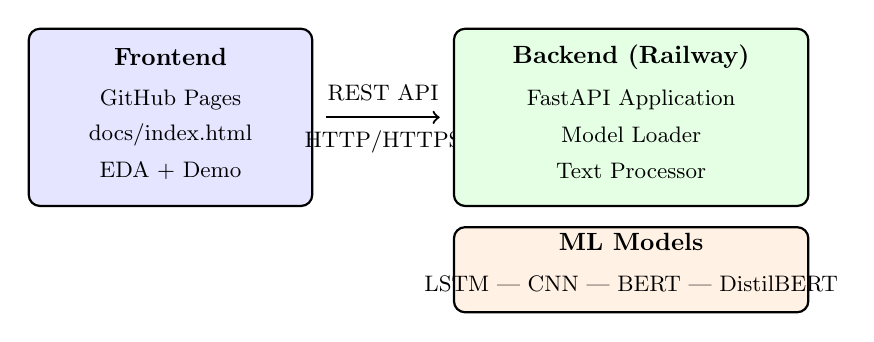
\begin{tikzpicture}[scale=0.9, transform shape]
        % Frontend box
        \draw[thick, fill=blue!10, rounded corners] (0,0) rectangle (4,2.5);
        \node[font=\bfseries] at (2, 2.1) {Frontend};
        \node[font=\small] at (2, 1.5) {GitHub Pages};
        \node[font=\small] at (2, 1.0) {docs/index.html};
        \node[font=\small] at (2, 0.5) {EDA + Demo};
        
        % Arrow
        \draw[->, thick] (4.2, 1.25) -- (5.8, 1.25);
        \node[font=\small] at (5, 1.6) {REST API};
        \node[font=\small] at (5, 0.9) {HTTP/HTTPS};
        
        % Backend box
        \draw[thick, fill=green!10, rounded corners] (6,0) rectangle (11,2.5);
        \node[font=\bfseries] at (8.5, 2.1) {Backend (Railway)};
        \node[font=\small] at (8.5, 1.5) {FastAPI Application};
        \node[font=\small] at (8.5, 1.0) {Model Loader};
        \node[font=\small] at (8.5, 0.5) {Text Processor};
        
        % Models box
        \draw[thick, fill=orange!10, rounded corners] (6,-1.5) rectangle (11,-0.3);
        \node[font=\bfseries] at (8.5, -0.5) {ML Models};
        \node[font=\small] at (8.5, -1.1) {LSTM | CNN | BERT | DistilBERT};
    \end{tikzpicture}
    
    \vspace{0.5cm}
    \textbf{API Endpoints:} /api/health | /api/predict/lstm | /api/predict/cnn | /api/predict/all
\end{frame}

% ============================================================================
% SLIDE 9: Deployment
% ============================================================================
\begin{frame}{Deployment}
    \begin{columns}
        \begin{column}{0.5\textwidth}
            \textbf{Backend (Railway.app):}
            \begin{itemize}
                \item NIXPACKS builder
                \item Python 3.11
                \item Uvicorn ASGI server
                \item Auto-restart on failure
                \item Environment variables for config
            \end{itemize}
            
            \vspace{0.3cm}
            \textbf{Model Files:}
            \begin{itemize}
                \item best\_cnn\_model.pth
                \item best\_lstm\_model.pth
                \item best\_bert\_model/
                \item best\_distilbert\_model/
                \item vocab.json
            \end{itemize}
        \end{column}
        \begin{column}{0.5\textwidth}
            \textbf{Frontend (GitHub Pages):}
            \begin{itemize}
                \item Static files in docs/
                \item Automatic deployment
                \item CORS configuration
            \end{itemize}
            
            \vspace{0.3cm}
            \textbf{Utility Scripts:}
            \begin{itemize}
                \item prepare\_for\_railway.py
                \item download\_models.py
            \end{itemize}
            
            \vspace{0.3cm}
            \textbf{Documentation:}
            \begin{itemize}
                \item Training notebooks
                \item Deployment guides
                \item API documentation
            \end{itemize}
        \end{column}
    \end{columns}
\end{frame}

% ============================================================================
% SLIDE 10: Conclusion & Future Work
% ============================================================================
\begin{frame}{Conclusion \& Future Work}
    \begin{columns}
        \begin{column}{0.5\textwidth}
            \textbf{Achievements:}
            \begin{itemize}
                \item[$\checkmark$] 4 trained models
                \item[$\checkmark$] Full web interface
                \item[$\checkmark$] Model comparison
                \item[$\checkmark$] Attention visualization
                \item[$\checkmark$] Production deployment
                \item[$\checkmark$] Comprehensive docs
            \end{itemize}
        \end{column}
        \begin{column}{0.5\textwidth}
            \textbf{Future Improvements:}
            \begin{itemize}
                \item Real attention weights from transformers
                \item Ensemble methods
                \item User prediction history
                \item Batch text processing
                \item Results export
                \item Monitoring \& logging
            \end{itemize}
        \end{column}
    \end{columns}
    
    \vspace{0.5cm}
    \centering
    \textbf{\large Thank you!}
    
    \vspace{0.3cm}
    \small{Repository: github.com/MichailLepin/Fake-News-Classifier}
\end{frame}

\end{document}

